%
% intro
% @author Tobias Weber <tweber@ill.fr>
% @date mar-2021
% @license see 'LICENSE' file
%

\chapter{Introduction}
\label{ch:intro}
In this first chapter, we introduce some basic concepts of neutron scattering and shortly present two types of
instruments typically found at research reactors (section \ref{sec:instruments}). A special emphasis is put
on triple-axis spectrometers (TAS) as the work-horse of inelastic neutron scattering. Finally, we summarise
the current state of autonomous experimentation (section \ref{sec:autonomous}).


\section{A brief history of neutron physics \label{sec:neutrons}}

The history of neutron physics begins in 1932 with the discovery of the neutron by James Chadwick, who used
alpha particles (helium nuclei) to bombard a beryllium-9 sample, thereby producing carbon-12 and one neutron
per reaction \cite[p. 1]{Jacrot2021}. The neutron that was created in this way was found to have a mass similar
to the proton ($m_n = 1.675\cdot10^{-27}\,\mathrm{kg}$, $m_p = 1.673\cdot10^{-27}\,\mathrm{kg}$), but, as the
name implies, no charge was detected \cite[p. 2]{Squires2012}. The absence of a charge makes the neutron very
useful for science, as it is subject to purely nuclear interactions with atomic nuclei, without any electrostatic
repulsion, for example by the electron hull \cite[p. 1]{Squires2012}.

In 1939, Otto Hahn used a Chadwick-type neutron source to irradiate uranium isotopes in an attempt to produce
heavy trans-uranium elements \cite{wiki_fission}. The measurements did not yield the expected results, because
instead of heavier elements, the experiment produced lighter elements. This was interpreted by Lise Meitner as
a splitting of the uranium nucleus, marking the discovery of nuclear fission \cite{wiki_fission}. A typical possible
channel of a fission reaction is the decay of uranium-235 into baryum-144 and krypton-89, where two to three
neutrons are produced by each reaction in addition to the daughter nuclei and energy \cite{wiki_fission}.

In 1942, Enrico Fermi made use of the excess neutrons that are obtained by each fission reaction to produce a
continuous, self-sustaining chain reaction in the first artificial nuclear reactor, the
\textit{Chicago Pile-1}~\cite[p.1]{Jacrot2021}.
It is interesting to note that while \textit{Chicago Pile-1} was the first \textit{artificial} nuclear reactor,
it was not the first one, strictly speaking. The first \textit{natural} reactor was discovered to have run more
than 1.5 billion years ago in Oklo, Gabun, at an average power of about 100 kW for a period of half a million
years \cite{wiki_oklo}.

The first research reactor, having a power of 3.5 MW~\footnote{As research reactors do not produce electricity,
the given numbers refer to thermal powers.} and being used for studies in solid-state physics, was built in
Oak Ridge, USA, in 1943, shortly after Fermi's pile \cite[p. 3]{Jacrot2021}.
Here, first neutron scattering experiments were performed by Clifford Shull using a two-axis diffractometer \cite[pp. 3, 37]{Jacrot2021}.

From there on, science advanced fast, and several centres dedicated to neutron research were founded around the world.
A selection of research reactors in operation today include the 20 MW \textit{Forschungsreaktor M\"unchen II}~\cite{web_mlz}
(FRM-II) at the Heinz-Maier-Leibnitz-Zentrum in Germany,
the 20 MW reactor at the NIST Center for Neutron Research~\cite{web_nist} (NCNR),
the 85 MW \textit{High Flux Isotope Reactor}~\cite{web_oakridge} (HFIR) at the Oak Ridge National Laboratory,
both based in the United States,
and the reactor of the Institut Laue-Langevin~\cite{web_ill} (ILL) in France, which - at 58 MW - is the most
powerful neutron source used for science in Europe.

Studying the structure and dynamics of crystals is made possible since neutrons emerging from the reactor can be
slowed down (moderated) into energy regions where their de Broglie wavelength $\lambda = h/p$ \cite[p. 89]{Gross2012}
corresponds to typical inter-atomic distances in crystal unit cells, which is of the order of 1 \AA{}ngstr\"om,
i.e. $10^{-10}$ m \cite[pp.1,3]{Squires2012}. In the formula, $p$ denotes the neutron momentum and $h$ Planck's constant.
Such a slowing-down of neutrons is usually performed using a secondary moderator outside the reactor's main moderator --
which itself sustains the nuclear fission -- for example using liquid $\mathrm{D_2O}$ \cite[p. 82]{Jacrot2021}.
Here, neutrons are brought into a new thermal equilibrium by elastic collisions with the nuclei of the moderator's
atoms \cite[p. 30]{Stacey2007}, i.e. the neutrons take the temperature and thus energy of the surrounding material.



\section{Instruments for neutron scattering \label{sec:instruments}}

While a modern research reactor houses a multitude of different instrument types, among them time-of-flight,
back-scattering and spin-echo spectrometers, furthermore Larmor, Laue and small-angle diffractometers (see, for example, Ref. \cite{ExperimentalFacilites} for an explanation of these types of instrument), in
this section, we instead want to shortly present the most basic types of instrument, the two-axis diffractometer
and the triple-axis spectrometer. Together, the discovery of these two instruments by Clifford Shull and Bertram Brockhouse,
respectively, was awarded the 1994 Nobel Prize in Physics~\cite{web_nobel1994}.
A comprehensive introduction into these instruments, especially triple-axis spectroscopy, can be found in the
book by G. Shirane \cite{Shirane2002}. An advanced treatment of neutron scattering theory is given by
G. L. Squires \cite{Squires2012}.


\subsection{Two-axis diffractometers}

A two-axis diffractometer is used for determining the static structure of crystals \cite[pp. 89f]{Gross2012},
which are here typically provided in powder form, but can also be single-crystals.
It is the single most fundamental kind of machines in the field of
neutron scattering at research reactors. This instrument type consists of a single-crystal (meaning it comprises one
single grain), which is called ``monochromator'' and named after its function to pick out one specific wavelength,
$\lambda_i$, from the polychromatic neutron beam coming from the reactor core or from one of its moderators.
The physical principle behind wavelength selection is Bragg reflection \cite[p. 68]{Gross2012} \cite[p. 13]{Shirane2002},
\begin{equation}
	\label{eq:bragg}
	n \cdot \lambda_i \ =\  2 d \cdot \sin\left( \theta_M \right),
\end{equation}
with $\lambda_i$ being the neutron wavelength, $d$ the spacing of the crystal lattice planes from which scattering
takes place, $\theta_M$ half the monochromator scattering angle and $n$ the order of the reflection. A graphical
interpretation of Eq. \ref{eq:bragg} is depicted in Fig. \ref{fig:braggscattering}.

\begin{figure}[htb]
	\centering
	\includegraphics[width=0.35\textwidth]{figures/bragg.pdf}
	\caption[Bragg scattering.]{
		Bragg scattering on crystal planes having a spacing $d$. An incoming parallel neutron beam is reflected at an
		angle $2 \cdot \theta_M$ on both the upper and lower crystal plane, leading to a path difference of
		$2d \sin\theta$ between the beams. If the path difference is an integer multiple of the neutron wavelength,
		$\lambda_i$, the beams interfere constructively, yielding a strong reflection.
		Figure drawn after \cite[p. 68, Fig. 2.7]{Gross2012}. }
	\label{fig:braggscattering}
\end{figure}

The resulting monochromatic beam with the wavelength $\lambda_i$ and wavevector $\underline{k}_i$ is Bragg-scattered
a second time, this time from a sample powder containing small crystallites. Diffractometers typically contain hundreds
of neutron detectors surrounding the sample and picking up diffracted neutrons at a whole range of scattering angles
$2 \theta_S$. The scattering angles define the momentum transfer from the neutron to the sample as \cite[p. 11]{Shirane2002}
\begin{equation}
	\label{eq:Q}
	\hbar \underline{Q} \ =\  \hbar \left( \underline{k}_i - \underline{k}_f \right),
\end{equation}
where the two wavevectors $\underline{k}_i$ and $\underline{k}_f$ point along the propagation directions of the neutrons
before and after scattering from the sample, respectively. They both have the same magnitudes for diffraction, namely
$k_{i,f} = 2\pi / \lambda_i$ and are rotated by $2\theta_S$ from one another, see Fig. \ref{fig:diffraction} for a visualisation.
The symbol $\hbar$ denotes the reduced Planck's constant, $\hbar = h / \left( 2\pi \right)$.

\begin{figure}[htb]
	\centering
	
\includegraphics[width=0.35\textwidth]{figures/diffraction.pdf}
	\caption[Neutron diffraction.]{
		Principle of neutron diffraction. A polychromatic neutron beam coming from the reactor core is Bragg-scattered
		from the monochromator (M), picking out a single wavelength $\lambda_i$ and corresponding wavevector $\underline{k}_i$.
		The monochromatic beam is next scattered on the sample (S) at an angle $2\theta_S$, defining the direction of a
		wavevector $\underline{k}_f$. The momentum transferred from the neutron to the sample is given by Eq. \ref{eq:Q}
		as the difference of the two wavevectors.}
	\label{fig:diffraction}
\end{figure}

By the intensity of the sample's Bragg reflections, each of which appears at a different scattering angle $2\theta_S$
and thus momentum transfer $\hbar \underline{Q}$, the so-called static nuclear structure factor \cite[p. 25]{Shirane2002}
can be reconstructed.
Absences of Bragg peaks determine the crystal symmetry given by its space group \cite[pp. 13-15]{Gross2012}.
Together, they determine the structural build-up of the crystal.


\subsection{Triple-axis spectrometers}

In a two-axis diffractometer the scattering angle from a sample defines a momentum $\hbar \underline{Q}$ which is
transferred from the the neutron to the sample. It does not allow to select a sample-neutron energy transfer,
which is given by the de Broglie equation as \cite[p. 89]{Gross2012} \cite[p. 11]{Shirane2002}
\begin{equation}
	\label{eq:E}
	E \ =\ E_i - E_f \ =\ \frac{\left( \hbar k_i \right)^2}{2 m_n} - \frac{\left( \hbar k_f \right)^2}{2 m_n}.
\end{equation}
The constant $m_n$ is the neutron mass, for elastic scattering $k_i = k_f$.
The data obtained from such an instrument is instead integrated over all possible energy transfers.
This is no problem in practice, because elastic scattering, i.e. scattering with no energy transfer,
is usually many orders of magnitude stronger than inelastic scattering and any inelastic contribution
would not hide the elastic signals used for crystal structure determination.

Complementary to the two-axis instrument, a triple-axis spectrometer (TAS) is usually not used to study structures,
but instead measures the dynamics of the sample crystal \cite[pp. 214-215]{Gross2012}.
The samples used at TAS are usually in single-crystalline form.
At TAS machines, we are thus mainly interested in non-zero energy transfers, i.e. the cases when neutrons scattering from the
sample crystal excite collective modes. These modes typically comprise vibrations of the crystal's nuclei, called phonons,
which can be imagined as quantised sound waves \cite[pp. 123-137]{Shirane2002}. Another typical example includes the
coupled motions of the atom hull's electron spins, which are named spin-waves or magnons \cite[pp. 137-144]{Shirane2002}.

As the name implies, the difference of the TAS set-up compared to the two-axis diffractometer is one additional axis.
Having passed the sample, the neutrons may have changed their energy and thus wavelength and magnitude of the wavevector.
A further single-crystal is placed in the neutron path between the sample and the detector. Bragg scattering on this crystal
allows the detection of the neutron wavelength $\lambda_f$ after the sample, which remained unknown in the diffractometer.
Since we also know the incoming wavelength $\lambda_i$ before the scattering event at the sample, we can calculate the
transferred energy as given by Eq. \ref{eq:E}. This additional crystal and the corresponding instrument axis are named ``analyser''.
Fig. \ref{fig:spectroscopy} visualises the principles of the instrument, Fig. \ref{fig:thales} shows a typical triple-axis
instrument with its three axes, namely the monochromator in the right-hand side of the picture, the sample and the analyser
with the attached detector.

\begin{figure}[htb]
	\centering
	
\includegraphics[width=0.4\textwidth]{figures/spectroscopy.pdf}
	\caption[Neutron spectroscopy.]{
		Principle of neutron spectroscopy. A polychromatic neutron beam coming from the reactor core is Bragg-scattered
		from the monochromator crystal (M), picking out a single wavelength $\lambda_i$ and wavevector $\underline{k}_i$.
		The monochromatic beam is next scattered on the sample (S) at an angle $2\theta_S$, defining a wavevector $\underline{k}_f$.
		The magnitude of $\underline{k}_f$ and thus $\lambda_f$ is determined by Bragg-scattering on the analyser crystal (A).
		The momentum and energy transfers are given by Eqs. \ref{eq:Q} and \ref{eq:E}, respectively. }
	\label{fig:spectroscopy}
\end{figure}

\begin{figure}[htb]
	\centering
	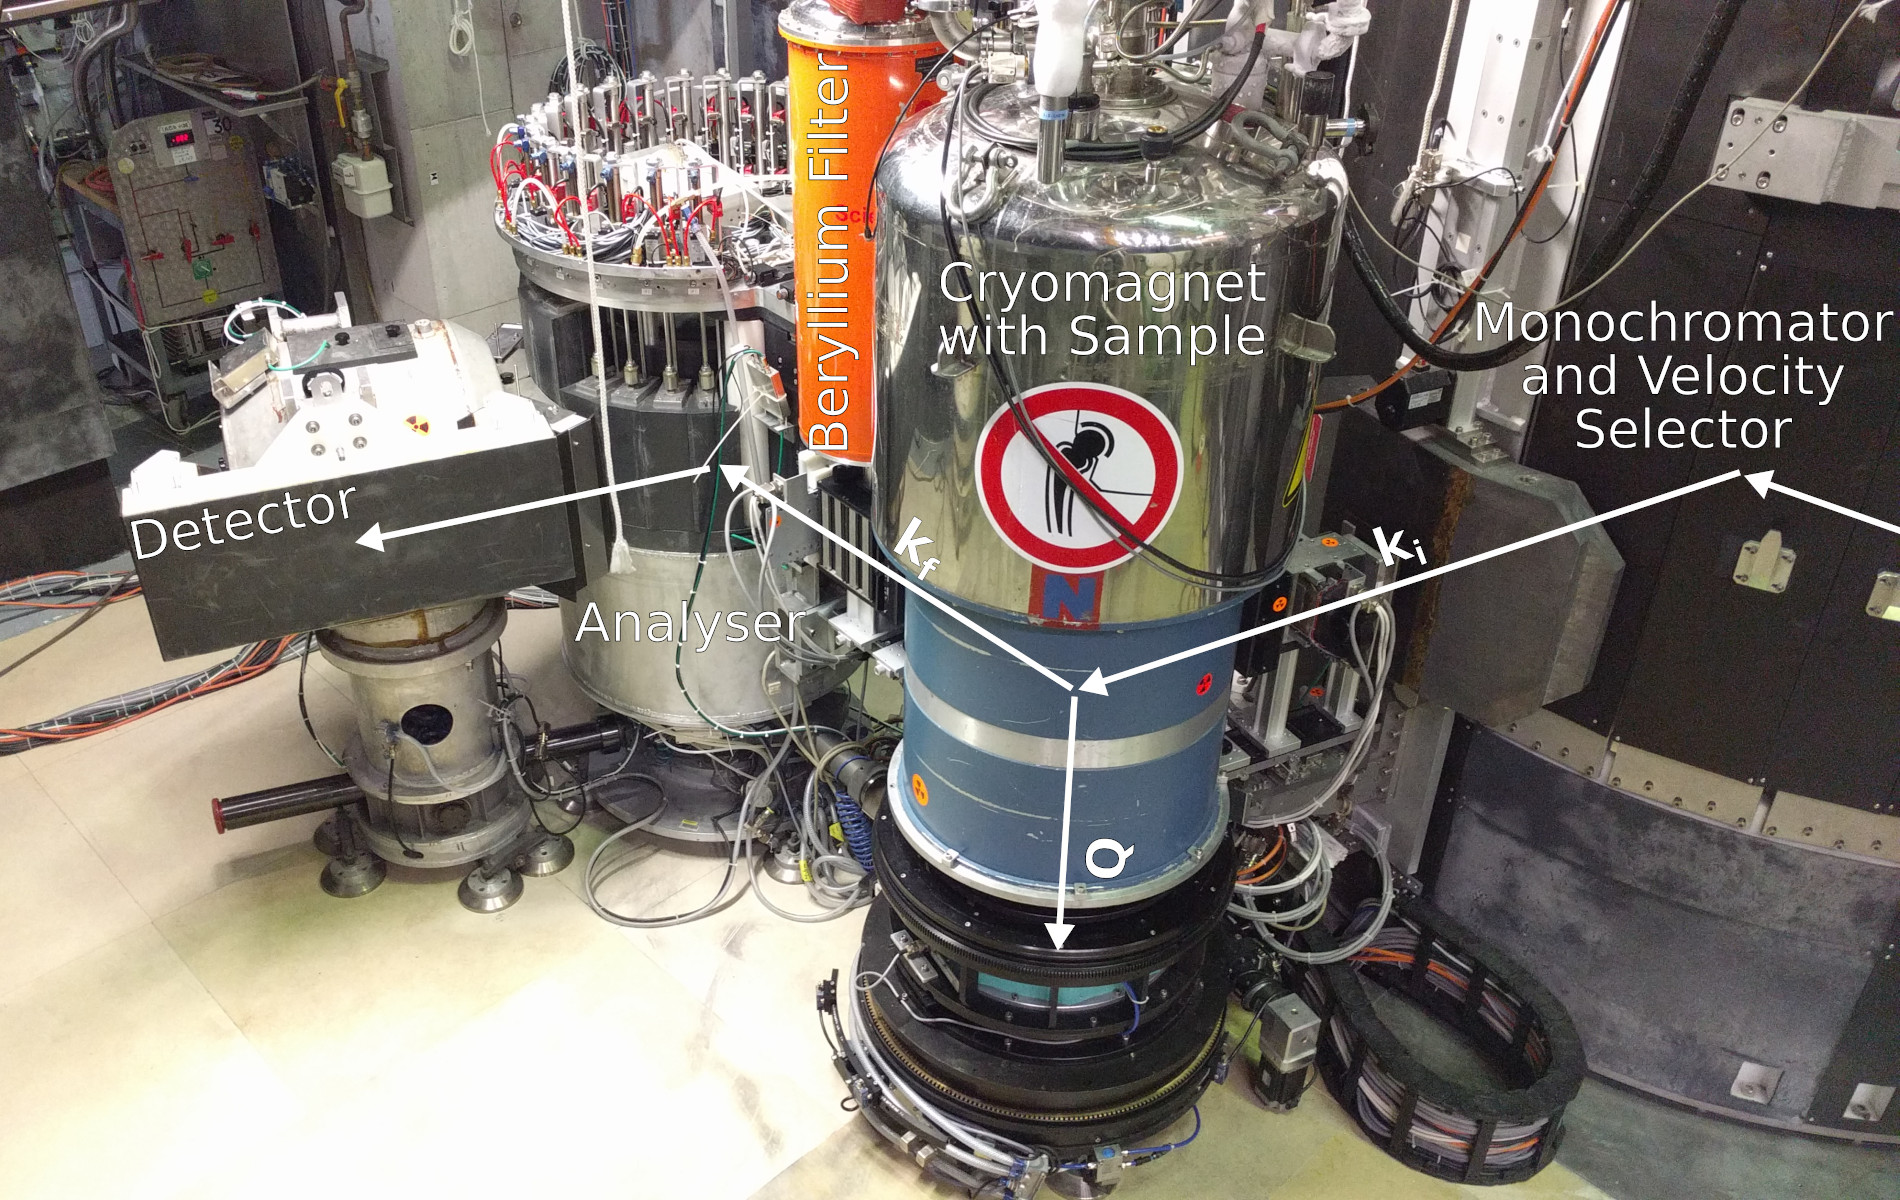
\includegraphics[width=0.75\textwidth]{figures/thales.jpg}
	\caption[The Thales instrument at the ILL.]{
		The triple-axis spectrometer \textit{Thales} \cite{thales} at the Institut Laue-Langevin in Grenoble, France.
		The neutron path from the reactor to the detector is marked as white arrows. The momentum transfer, 
		$\hbar \underline{Q}$, is also shown.
		This picture is reproduced from the supplementary information of Ref. \cite{skxpaper}.}
	\label{fig:thales}
\end{figure}



\section{Autonomous experiments \label{sec:autonomous}}

Up until the end of 2019, TAS experiments usually required external scientists to stay at the research reactor for
typically one week and conduct the experiment together with the instrument's responsible scientists. Specifically
at the Institut Laue-Langevin (ILL), there had already been attempts \cite{Song2020} of the instrument control
and scientific computing groups to convince the instrument scientists of the benefits of instrumentation with full- or
semi-autonomous as well as remote control. Nevertheless, the impact had been limited.
Virtual experiments, on the other hand, had already been established in the simulation of actual experiments and in their
planning phase. Noteworthy software systems are \textit{McStas} \cite{McStas2020, McStas2021}, a neutron ray-tracing software based on the
Monte-Carlo method, simulating a large number of random neutrons and their interaction with various neutron-optical components,
as well as the software \textit{vTAS} \cite{vTAS2013}, which simulates the angles and crystal coordinates of a triple-axis
instrument and also provides support for calculating collisions with walls.

The situation changed significantly with the Covid-19 pandemic. Receiving visiting scientists from other countries had
not been possible anymore, or only to a very limited degree. Instead, remote experimentation and instrument control has
now become the new norm, with users connecting to a web interface from which the experiment can be planned and data can
be analysed~\cite{web_ill_visa}.
Discussions with instrument scientists take place via web-cams that have been installed at every instrument.

At the same time, the idea to automate manual tasks at instruments using algorithms and artificial intelligence has
gained significant traction, with first autonomous experiments being attempted at the ILL's spectroscopy group
\cite{web_ill_autonomous2020, Noack2021}.

As part of the current drive towards autonomous experimentation at the ILL, the goal of the present work is the design
and implementation of a software tool which enable an automatic pathfinding for TAS instruments. Pathfinding
is necessary for the instrument to circumvent obstacles in its way and for safe, collision-free movement close to walls.
Currently, this task has to be performed by the instrument scientists before each new scan series in a time-consuming fashion.
The current approach requires the instrument to be driven along the programmed scan path, but without measuring and with
the neutron beam from the reactor closed.
The scientist has to stay in the instrument space and watch the instrument as it moves to every scan position.
A manual stop has to be initiated when the instrument would collide with a wall, with itself, or when the rotation of one
of the axes would pull out a cable or tube.

An early attempt at automatic collision prevention and pathfinding for a triple-axis spectrometer can be found in
the 2006 work by M\"uhlbauer and Hradil \cite{Muehlbauer2006}, but their method is based on a simple grid search and thus
does not result in paths which keep the farthest distance to obstacles. A reason for such a solution might be
that computing power was not sufficient at that time to calculate the mesh of possible paths as it is 
done with the algorithms to be presented in the current work.



\section{Summary}

This chapter provided a short glance at neutron physics and the types of instrument typically used at research
reactors, with special emphasis on the triple-axis spectrometer. The complexity of the movement of these kind of
instruments necessitate the use of a pathfinding system for a more effective set-up of measurements.
In the next chapter, we will introduce the coordinate systems used in crystallography and at TAS instruments,
and show how one set of coordinates transforms into the other.
